\section{Numerical Mathematics Fundamendals}


\subsection{Problem 4.8}


\begin{figure}[!ht]
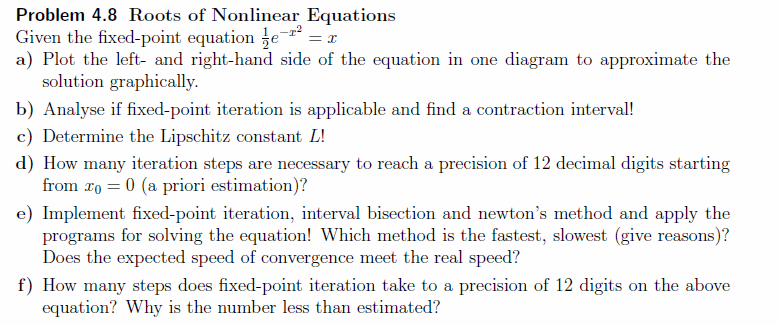
\includegraphics[width=1\textwidth]{chapters/images/desc-4-8}
\end{figure}


X

\begin{lstlisting}[caption=todo]

def fFixed(x):
	return 0.5 * pow(math.e, -pow(x, 2));


def fFixedDerived(x):
	return -pow(math.e, -pow(x, 2)) * x;


def f(x):
	return fFixed(x) - x;


def fDerived(x):
	return fFixedDerived(x) - 1;

\end{lstlisting}

Y


\subsubsection{a)}

X

\begin{lstlisting}[caption=todo]

xses = [];
fLeft = [];
fRight = [];

for i in range(200):
	x = (i / 100.0) - 1;
	
	xses.append(x);
	fLeft.append(fFixed(x));
	fRight.append(x);


plt.plot(xses, fLeft);
plt.plot(xses, fRight);
plt.xlabel('x');
plt.ylabel('y');
plt.show();


\end{lstlisting}


results:



\begin{figure}[!ht]
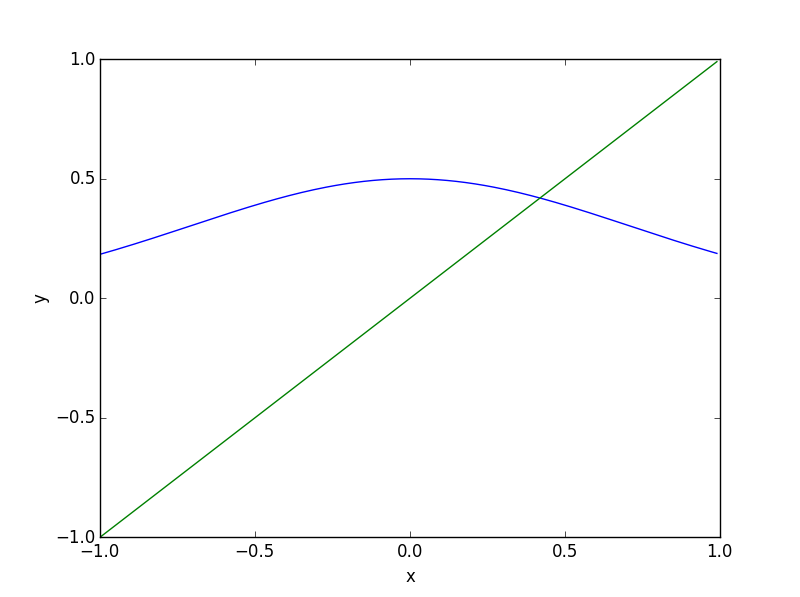
\includegraphics[width=1\textwidth]{chapters/images/figure-4-8-a}
\caption{todo}
\end{figure}

graphical solution: little less than 0.5



\subsubsection{b)}

fixed-point iteration is applicable since 0 < L < 1 (see c))
contraction interval: [0, 1] -> [0, 1]




\subsubsection{c)}

X

\begin{lstlisting}[caption=todo]

# -0.70711 and 0.70711 are roots of the 2nd derivative of f
lipschitz = abs(fFixedDerived(0.70711));

print("L = " + str(lipschitz));

\end{lstlisting}


results:

\begin{lstlisting}[caption=Result of 1.1 a), keywordstyle=\color{black}]
L = 0.428881942471
\end{lstlisting}

X



\subsubsection{d)}

X

\begin{lstlisting}[caption=todo]

steps = 0;
err = 1;
xdiff = f(0);

while err > 1e-12:
	steps = steps + 1;
	err = (pow(lipschitz, steps) / (1 - lipschitz)) * xdiff;

print(str(steps) + " iteration steps required");

\end{lstlisting}


results:

\begin{lstlisting}[caption=Result of 1.1 a), keywordstyle=\color{black}]
33 iteration steps required
\end{lstlisting}


\subsubsection{e)}

\begin{lstlisting}[caption=todo]

def isPreciseEnough(val, goal, precision):
	f = pow(10, precision);

	return math.floor(val * f) == math.floor(goal * f);


def getFixedPoint(x0, goal, precision):
	x = x0;
	steps = 1;
	
	while steps < 100:
		x = fFixed(x);
		
		if (isPreciseEnough(x, goal, precision)):
			break;
		
		steps = steps + 1;
	
	return steps;


def mySign(x):
	return -1 if x < 0 else 1;


def getRootBisection(pXA, pXB, goal, precision):
	xa = pXA;
	xb = pXB;
	xm = -1;
	steps = 1;
	
	while steps < 100:
		xm = xa + (xb - xa) / 2.0;
		
		if (isPreciseEnough(xm, goal, precision)):
			break;
		
		if mySign(f(xa)) != mySign(f(xm)):
			xb = xm;
		else:
			xa = xm;
		
		steps = steps + 1;
	
	return steps;


def getRootNewton(x0, goal, precision):
	x = x0;
	steps = 1;
	
	while steps < 100:
		fD = fDerived(x);
		
		if abs(fD) < 0.00001: fD = 0.00001;
		
		x = x - float(f(x) / float(fD));
		
		if (isPreciseEnough(x, goal, precision)):
			break;
		
		steps = steps + 1;
	
	return steps;


def getTime():
	return time.time();


def printTimeDiff(startTime, endTime):
	averageMS = round((endTime - startTime) / 10.0, 5);
	print("average time taken: " + str(averageMS) + " milliseconds");


def findRoot(type, goal, precision, p1 = 0, p2 = 0):
	startTime = getTime();
	
	steps = 0;
	
	for i in range(10000):
		param1 = p1 + 0.000001 * math.sin(i * 7);
	
		if (type == 0): steps = getFixedPoint(param1, goal, precision);
		elif (type == 1): steps = getRootBisection(param1, p2, goal, precision);
		else: steps = getRootNewton(param1, goal, precision);
	
	print("steps taken: " + str(steps));
	printTimeDiff(startTime, getTime());



def getFixedPointRec2(x, maxSteps, stepsTaken):
	newX = fFixed(x);
	
	if stepsTaken < maxSteps:
		return getFixedPointRec2(newX, maxSteps, stepsTaken + 1);
	else:
		return newX;


def getFixedPointRec1(x0, maxSteps):
	return getFixedPointRec2(x0, maxSteps, 1);


fP33 = getFixedPointRec1(0, 100);

precision = 6;
print("correct digits required: " + str(precision));

print("fixed point iteration:");
findRoot(0, fP33, precision, 0, -1);

print("interval bisection:");
findRoot(1, fP33, precision, 0, 1);

print("newton's method:");
findRoot(2, fP33, precision, 0, -1);

precision = 12;
print("correct digits required: " + str(precision));

print("fixed point iteration:");
findRoot(0, fP33, precision, 0, -1);

print("interval bisection:");
findRoot(1, fP33, precision, 0, 1);

print("newton's method:");
findRoot(2, fP33, precision, 0, -1);

precision = 18;
print("correct digits required: " + str(precision));

print("fixed point iteration:");
findRoot(0, fP33, precision, 0, -1);

print("interval bisection:");
findRoot(1, fP33, precision, 0, 1);

print("newton's method:");
findRoot(2, fP33, precision, 0, -1);

\end{lstlisting}


results:

\begin{lstlisting}[caption=Result of 1.1 a), keywordstyle=\color{black}]
correct digits required: 6
fixed point iteration:
steps taken: 14
average time taken: 0.0382 milliseconds

interval bisection:
steps taken: 17
average time taken: 0.0914 milliseconds

newton's method:
steps taken: 4
average time taken: 0.0237 milliseconds

correct digits required: 12
fixed point iteration:
steps taken: 27
average time taken: 0.1185 milliseconds

interval bisection:
steps taken: 40
average time taken: 0.2703 milliseconds

newton's method:
steps taken: 4
average time taken: 0.0321 milliseconds

correct digits required: 18
fixed point iteration:
steps taken: 35
average time taken: 0.1501 milliseconds

interval bisection:
steps taken: 51
average time taken: 0.3547 milliseconds

newton's method:
steps taken: 5
average time taken: 0.0377 milliseconds
\end{lstlisting}

Newton's method is the fastest because it also utilizes the first derivative of the function.

Interval bisection is the slowest because by always using the middle of the interval as a bound, it reaches the root the slowest.




\subsubsection{f)}

27 steps were needed instead of the estimated 33 steps. It took less steps because the a priori estimation always asumes the worst case scenario.


